\normaltrue
\correctionfalse

%\UPSTIidClasse{12} % 11 sup, 12 spé
%\newcommand{\UPSTIidClasse}{12}

\exer{Poutre encastrée $\star$ \label{RDM:05:def:542}}
\setcounter{question}{0}%\UPSTIcompetence[2]{C2-10}
\marginnote{\xpComp{RDM}{05}}
\index{Compétence C2-10}
\index{Compétence RDM-05}
\index{Torseur de cohésion}
\index{Déformée}

\ifcorrection
\else
\marginnote{\textbf{Pas de corrigé pour cet exercice.}}
\fi

On donne la poutre suivante. 



\marginnote{
\begin{itemize}
\item $\vect{F}=-F\vect{y}=-2000\vect{y}$;
%\item Poutre IPE 80;
\item $I_{G_z} = \SI{801400}{mm^4}$;
\item $E = \SI{200000}{MPa}$;
%\item $G = \SI{80000}{MPa}$;
\item $L= \SI{1}{m}$.
\end{itemize}}

\begin{figure}[H]
\centering
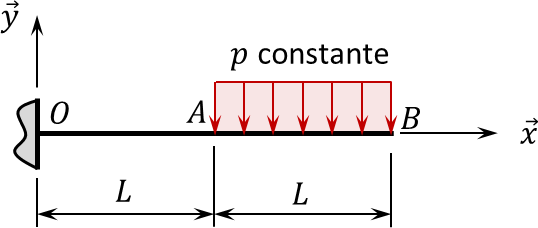
\includegraphics[width=.7\linewidth]{542}
%\caption{\label{61_01} Loi de commande de vitesse en trapèze}
\end{figure}

\question{Exprimer l'équation de la déformée de la poutre.}
\ifprof
%
%L'équation de la déformée est donnée par : $EI_{GZ}y''(x)=M_{fz}(x)$.
%
\textbf{Calcul du torseur de cohésion}

La poutre est composée de 2 tronçons :
\begin{itemize}
\item 1\ier tronçon : $\lambda\in[0,L]$
\item 2\ieme tronçon : $\lambda\in[L,2L]$
\end{itemize}

\textbf{1\ier tronçon}
\begin{itemize}
\item On isole la partie II.
\item BAME : 
\begin{itemize}
\item $\torseurstat{T}{I}{II}$
\item $\torseurstat{T}{p}{II}$
\end{itemize}
\item D'après le PFS, on a donc $\torseurstat{T}{I}{II} + \torseurstat{T}{p}{II} = \{0\}$ et donc 
$\torseurstat{T}{II}{I} =  \torseurstat{T}{p}{II}$.
\end{itemize}
On a donc $\forall \lambda\in[0,L]$, $\vectm{G}{F}{II}=  \left(3L/2-\lambda\right)\vect{x} \wedge - pL\vect{y} =- pL \left(\dfrac{3L}{2}-\lambda\right) \vect{z} $. 

Au final, $\torseurstat{T}{II}{I} = \torseurl{-pL\vect{y}}{- pL \left(\dfrac{3L}{2}-\lambda\right) \vect{z}}{G}$.


A SUIVRE...
%
%\textbf{2\ieme tronçon}
%
%$\forall \lambda \in [0,L]$, $\torseurstat{T}{II}{I} = \torseurl{\vect{0}}{\vect{0}}{G}$.
%
%\textbf{Calcul de la déformée sur le premier tronçon}
%
% $\forall x \in [L,2L]$, $EI_{GZ}y''(x)=-F\left(L-x\right) =-FL + Fx $ 
%et en intégrant $EI_{GZ}y'(x)= -FLx +\dfrac{1}{2}Fx^2+ c_1$ et  $EI_{GZ}y(x)= -\dfrac{1}{2}FLx^2 +F \dfrac{1}{6}x^3+ c_1x + c_2$.
%
%
%La liaison en $x=0$ étant une encastrement, on a $y(0)=0$ et $y'(0)=0$. 
%En conséquence, $c_2=0 $ et $c_1=0$.
%
%Au final, $EI_{GZ}y(x)= -\dfrac{1}{2}FLx^2 + \dfrac{1}{6}Fx^3 = Fx^2\dfrac{x - 3L}{6}$.
%
%
%On peut alors exprimer la flèche en $L$ : $EI_{GZ}y(L)= -\dfrac{ FL^3}{3}$.
%
%\textbf{Calcul de la déformée sur le second tronçon}
%
%$\forall x \in [L,2L]$, $EI_{GZ}y_2''(x)=0$ et en intégrant $EI_{GZ}y_2'(x)=c_3$ et $EI_{GZ}y_2(x)=c_3x + c_4$. 
%On a de plus $y(L) = y_2(L)$ et $y'(L) = y_2'(L)$. 
%
%D'une part, $F\dfrac{3L^2- 6L^2}{6}=c_3 $ et donc $c_3 =  -F\dfrac{ L^2}{2} $
%
%D'autre part, $FL^2\dfrac{L - 3L}{6}=-F\dfrac{ L^2}{2} L + c_4$ et $c_4 =  FL^2\dfrac{L - 3L}{6}+F\dfrac{ L^2}{2} L  = \dfrac{FL^3}{6}$.
%





\else

\fi

\question{Donner la valeur de la flèche maximale.}
\ifprof
\else
\fi



\ifprof
\begin{figure}[H]
\centering
%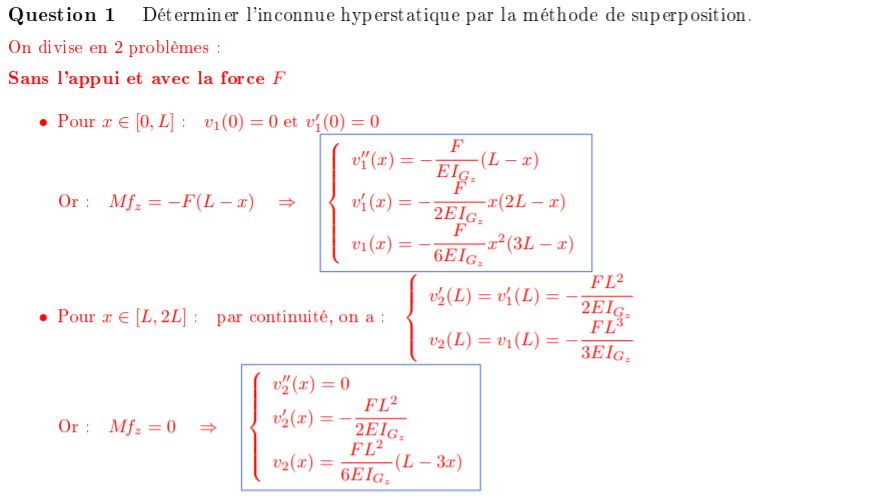
\includegraphics[width=\linewidth]{531_01_c}
%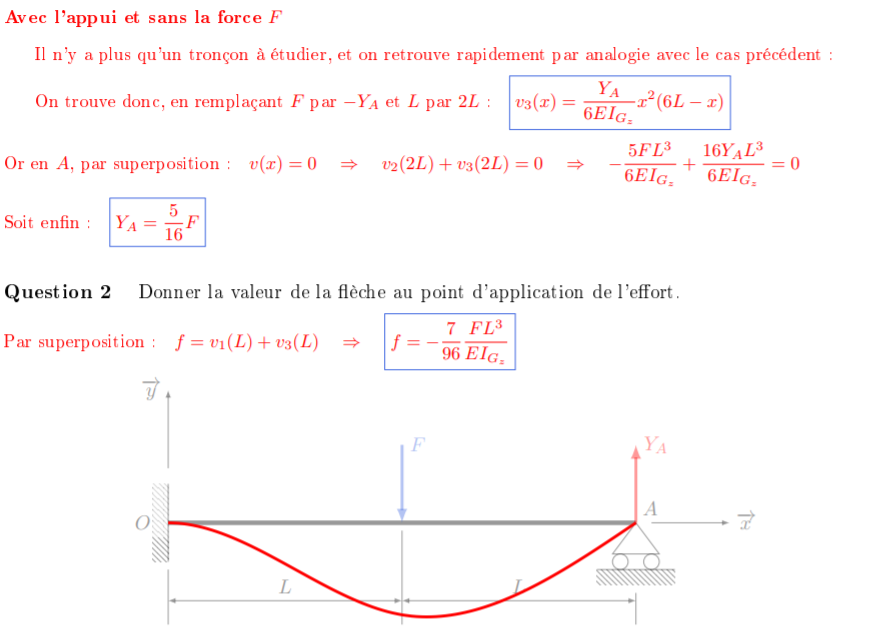
\includegraphics[width=\linewidth]{531_02_c}
\end{figure}
\else
%\footnotesize
%\begin{enumerate}
%  \item $\left(fp + Mp^2\right) Z(p)=S_h P_h(p)-S_e P_e(p) - \dfrac{Mg}{p}$
%    \item $Q_e(p)=\left(S_a - S_b \right)pL(p) + \dfrac{V_t}{B_e} p P_e(p)$ et $mp^2 L(p) = -rL(p)+\left(S_a-S_b\right) P_e(t)-f'pL(p)$.
%\end{enumerate}
%\normalsize


\marginnote{Corrigé voir \ref{RDM:05:def:542}.}

\fi